\documentclass[10pt]{article}
\usepackage{xeCJK}
\usepackage{amssymb}
\usepackage{amsthm}
\usepackage{mathtools}
\usepackage{amsmath}
\usepackage{amsfonts}
\usepackage{enumitem}
\usepackage{tikz-cd}
\usepackage{array}
\usepackage{makecell}
\usepackage{tabularx}
\usepackage[citestyle=authoryear,bibstyle=authortitle,sorting=ynt,backend=bibtex]{biblatex}
\usepackage{geometry}
\usepackage{multicol}
\usepackage{titling}
\usepackage{tcolorbox}
\addbibresource{template}
\geometry{a4paper,scale=0.9}
\newcounter{counter}
\newcommand{\counter}[1]{\refstepcounter{counter}\label{#1}\thecounter}

\setlength{\parindent}{0cm}
\setlength{\parskip}{1em}
\newcommand*{\qedfill}{\hfill\ensuremath{\blacksquare}}

\title{Testcast}
\author{}
\begin{document}
\maketitle
\begin{abstract}
\end{abstract}
\renewcommand{\setminus}{\mathbin{\backslash}}

\begin{tcolorbox}[colback=yellow]
左侧公式---Diophantine方程的示例:
\begin{align*} A X^{2}+B Y^{2} &=C \\ A X^{2}-B Y^{2} &=C \\ A X+B Y^{2} &=0 \end{align*}

右侧书籍封面图片《Diophantine Geometry》by Hindry \& Silverman
\end{tcolorbox}

对Diophantine几何,或更加特殊地,Diophantine方程的解的结构和特性的研究是一门源远流长的数学学科。

\begin{tcolorbox}[colback=yellow]
一张典型椭圆曲线的图像,例如
$$
-X^3+Y^2+X=0\quad\text{ or }\quad -X^3+Y^2+X-1\quad\text{ where }\quad (X,Y)\in\mathbb{R}^2
$$
下方标明曲线方程
\end{tcolorbox}

其中对一种特殊曲线——椭圆曲线——的研究是现代密码学发展过程中的重要一环。

\begin{tcolorbox}[colback=yellow]
\begin{enumerate}
\item 《Topology》 by Munkres
\item 《An Introduction to Commutative Algebra》 by Atiyah
\item 《The Arithmetics of Elliptic Curve》 by Silverman
\item 《Handbook of Elliptic and Hyperelliptic Curve Cryptography》 by Avanzi et al.
\end{enumerate}
\end{tcolorbox}

本系列内容将面向完成高中数学课程的用户介绍点集拓扑学、交换代数学、和古典代数几何学,并使用这些工具建立对椭圆曲线的理论体系,进而以综述该类曲线对现代密码学的影响。
在前4期内容中,我们将对点集拓扑学基础进行介绍。
应当注意的是,在观看视频的过程中用户应在需要时自行暂停视频。

\begin{tcolorbox}[colback=gray]
拓扑空间是具有如下结构$\mathcal{T}\subseteq\mathcal{P}(X)$的集合$X$:
\begin{enumerate}
\item $\emptyset,X\in\mathcal{T}$;
\item 任意属于$\mathcal{T}$的元素族的并集属于$\mathcal{T}$;
\item 有限属于$\mathcal{T}$的元素族的交集属于$\mathcal{T}$。
\end{enumerate}
\end{tcolorbox}

拓扑学是对拓扑空间和其间的连续映射进行研究的学科,我们首先定义拓扑空间。注意其中的$\mathcal{P}(-)$代表幂集。$\mathcal{T}$中的元素被称为“开集”。

\begin{tcolorbox}[colback=yellow]
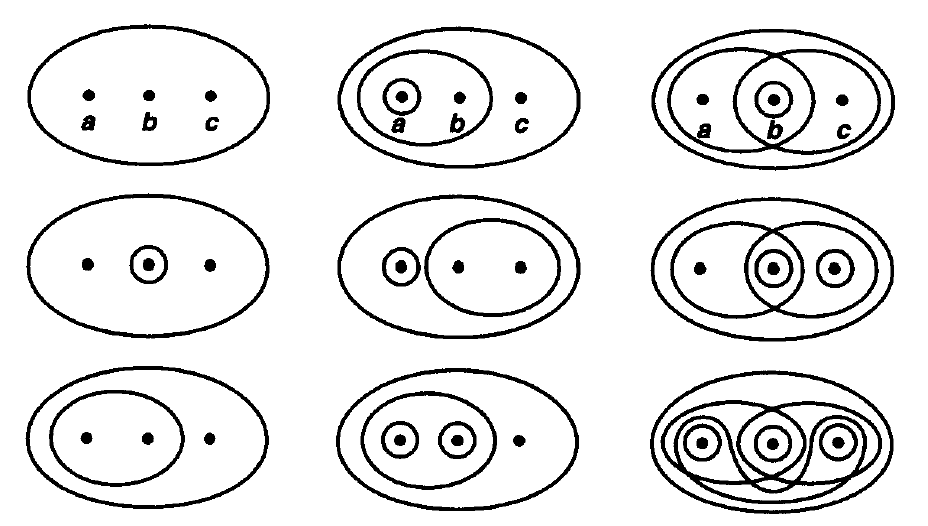
\includegraphics{1}
\end{tcolorbox}

考虑具有a,b,c三点的集合X,我们有很多可能的拓扑空间。这些拓扑空间结构以一种粗略的方式定义了“分离”或“粘合”的概念,并将其赋予集合$X$:考虑左上角的拓扑空间,包含$a,b,c$三点的开集族相同不可被以拓扑区分,在拓扑学的考虑范围内,它们是同一个点;而考虑右下角的拓扑空间,分别包含$a,b,c$三点的开集族不同,则这些点在拓扑意义上可区分。

\begin{tcolorbox}[colback=yellow]
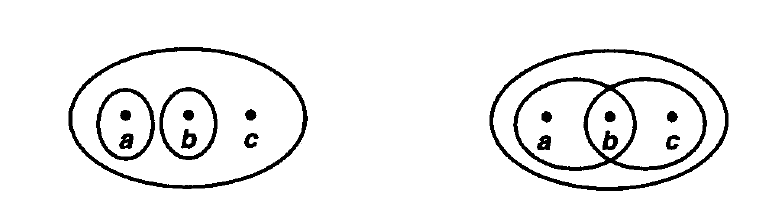
\includegraphics{2}
\end{tcolorbox}

但也有一些$\mathcal{T}\subseteq\mathcal{P}(X)$不满足全部的公理——它们不与$X$构成拓扑空间。

\begin{tcolorbox}[colback=yellow]
欧氏空间:$$\mathbb{E}^n=\underbrace{\mathbb{R}\times\cdots\times\mathbb{R}}_{n}$$
下方:空间直角坐标系图片
\end{tcolorbox}

我们回到熟悉的欧式空间。我们将定义一个其上的拓扑,使得它符合我们对欧氏空间原有的直觉。

\begin{tcolorbox}[colback=gray]
定义(欧氏拓扑). 对于$n<\infty$,能够被表示为
$$\bigcup_{i\in I}U_i$$
其中
$$(U_i)_j$$
为$\mathbb{R}$上开区间的形式的集合被称作欧氏拓扑中的开集,且欧氏拓扑不包含除上述外的任何其他开集。
\end{tcolorbox}

\begin{tcolorbox}[colback=yellow]
左右并排显示公式
$$D^2=\{\vec{x}\in\mathbb{R}^2\,\big|\,|x|<1\}$$
$$S^1=\{\vec{x}\in\mathbb{R}^2\,\big|\,|x|=1\}$$
其中左侧公式上方显示开球,右侧单位圆
\end{tcolorbox}

如图所示,左侧集合在$\mathbb{R}^2$中为开集,右侧为开集在$X$中的补集,被称为闭集。请用户在弹出的交互窗口中尝试探索一族如上所述的$U_i$来证明前者确为开集。

\section*{Reference}
\printbibliography
\end{document}
